% !TEX root = ./main.tex


\section{Bijlagen} % (fold)
\label{sec:bijlagen}

\appendix

\renewcommand{\thesubsection}{\Alph{subsection}}

\subsection{Prijsstrategieën} % (fold)
\label{sub:prijsstrategieën}

\paragraph{Klantengesprekken}

Via een tiental interviews nagaan welke waarde klanten aan je product hechten. 4 richtvragen:

\begin{itemize}
  \item Welke prijs is te duur?
  \item Welke te goedkoop?
  \item Welke is duur, maar zou je toch overwegen?
  \item Welke geeft je echt waar voor je geld?
\end{itemize}

Merk je dat de prijs die je zelf voor ogen had te duur is, dan is het beter om je waarde te verhogen dan je prijs te verlagen.

\paragraph{Break-even draaien}

Indien je een goed beeld hebt van je (potentiële) omzet, kosten en marges dan ken je de minimumprijs om je business levensvatbaar te maken. Let op: onderschat je kosten niet!

\paragraph{Buy vs. build}

Bij het bouwen van een applicatie:
\begin{enumerate}
  \item Onderzoek hoeveel het je klant zou kosten om de toepassing zélf van nul te bouwen.
  \item Reken daar jaarlijks 10\% van aan, dan geef je je klanten 10 jaar lang een topproduct dat bovendien continu evolueert, zonder dat hij zelf een grote investeringskost moet maken.
\end{enumerate}

\paragraph{Prijzenspectrum}

Plaats je concurrenten op een prijslijn én noteer er ook hun waarde (features en benefits) bij. Op die manier kan je jezelf in de markt positioneren. Hou deze methode voor op het einde, als een soort toetssteen.

\paragraph{Multiaxis pricing (prijs en waardes op klanten afstemmen)}

Je hanteert andere prijsmodellen afhankelijk van de klant. Deze prijsmodellen evolueren, ontstaan en doven uit. Niet iedereen heeft elke feature van je dienst/product nodig, of verwacht hetzelfde niveau van ondersteuning. Dit werkt drempelverlagend en biedt klanten een groeitraject. De meeste softwarebedrijven gebruiken deze drie assen.

\begin{itemize}
  \item Features: Meer functionaliteiten betekent een hogere prijs.
  \item Gebruikers: Klanten met veel gebruikers, zoals grote bedrijven, betalen meer. Maar de prijs per gebruiker gaat natuurlijk wel omlaag.
  \item Gebruik: Voor intenser gebruik – bijvoorbeeld meer schijfruimte – betaalt je klant iets meer.
\end{itemize}

Prijzen laten variëren is tried \& tested. Steeds meer dienstverleners (marketeers, consultants, coaches) maken er gebruik van maken. De gouden regel? Stem je prijs af op maximaal drie assen, want prijzen moeten begrijpelijk blijven.

\paragraph{Korting, pilootklanten, trialversie, freemium}

\begin{itemize}
  \item Kortingen: ideaal in een prijscompetitieve markt. Doe dit enkel tijdelijk. En verlaag je prijs niet, maar bied iets meer (bv. langer gebruik) in de plaats.
  \item Pilootklanten: ideaal voor b2b-omgevingen, waar je afspreekt met een klant om je product – of de bètaversie ervan – uit te proberen tegen een lagere prijs of zelfs tijdelijk gratis.
  \item Gratis trial: hou gratis tijdelijk – 14 dagen is zowat de standaard. Dat is meestal genoeg om een klant te overtuigen van je waarde, en om dus later een premiumversie te verkopen.
  \item Freemium: terwijl trials beperkt zijn in tijd, is bij het freemium-model enkel de naakte versie van je applicatie gratis. Extra gebruikers of features, in de premiumversie, zijn betalend. Zorg ervoor dat die extra’s echte meerwaarde bieden, anders kannibaliseer je je eigen aanbod.
\end{itemize}

% subsection prijsstrategieën (end)

\subsection{Business model} % (fold)
\label{sub:business_model}

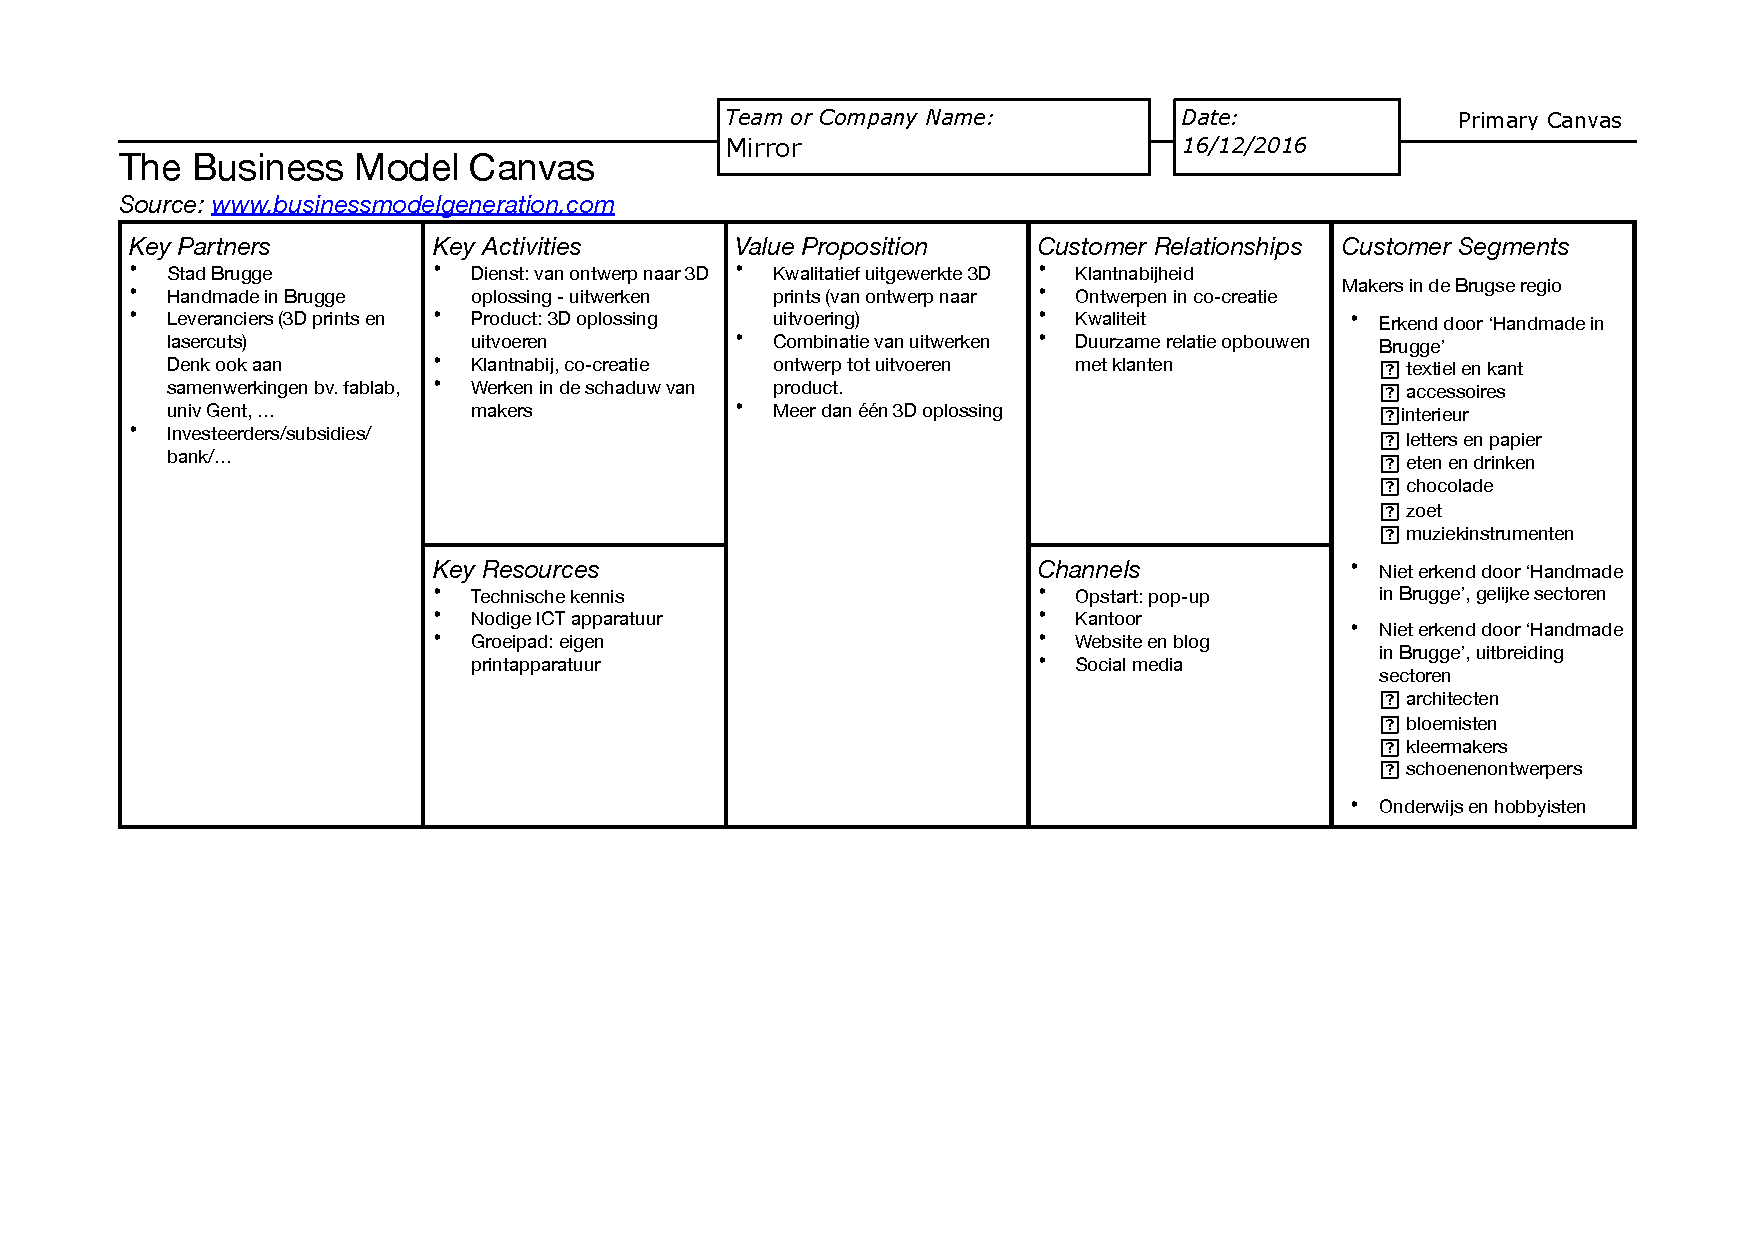
\includegraphics[width=\textwidth]{business-model.pdf}

% subsection business_model (end)

\subsection{Factuur} % (fold)
\label{sub:factuur}

Een factuur aangevraagd voor een lasercut van ca. $120cm^3$ bij een lokaal bedrijf.

\begin{centering}
  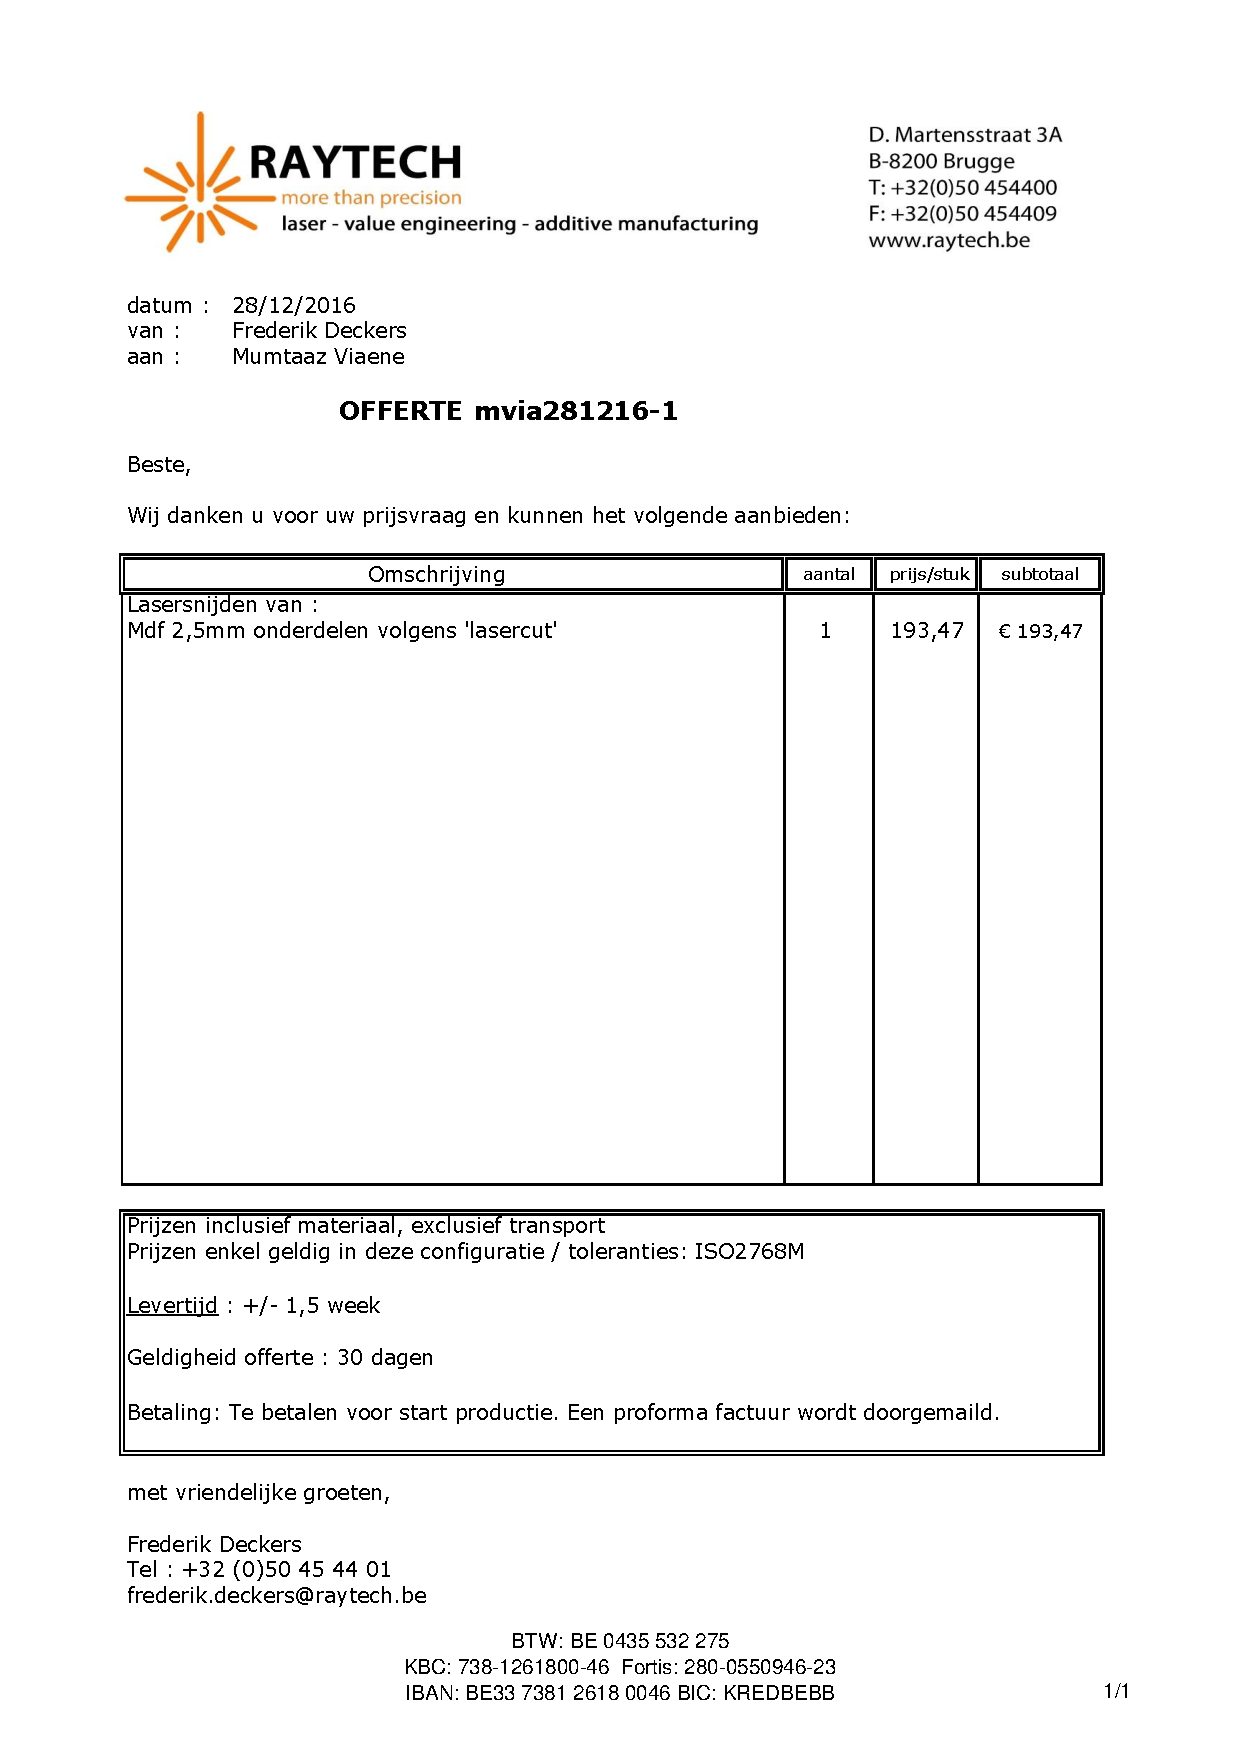
\includegraphics[height=0.9\textheight]{factuur.pdf}
\end{centering}

% subsection factuur (end)

\subsection{Door handmade in Brugge erkende makers} % (fold)
\label{sub:door_handmade_in_brugge_erkende_makers}

Informatie over door `Handmade in Brugge' erkende makers\cite{handmade-makers}.

\begin{longtabu} to \textwidth {XXX}
\caption{Textiel en kant}\label{table:erkende-makers-textiel}\\ \hline
Ilse Acke & Torhoutsestw 103-105, 8200 Brugge, 050 34 64 15, ilse.acke@telenet.be & Ilse Acke verweeft complexe grafische patronen, materialen en kleuren tot unieke sjaals, kussens en wandtapijten. Winnares van de Prijs voor Kunstambachten West-Vlaanderen 2013.Ilse Acke ontving van Handmade in Brugge de Prijs Innovatieve Maker 2015. \\ \hline
Arte / Grossé & L. Bauwensstraat 17, 8200 Brugge, 050 38 05 45, marc.schotte@artegrosse.be  & Meer dan 200 jaar vakmanschap in het vervaardigen en restaureren van religieuze kerkgewaden, kandelaars, lusters, wijwatervaten, kelken … \\ \hline
Chapellerie Baeckelandt & Ezelstraat 120, 8000 Brugge, 050 33 75 63,& Frédérique voorziet Bruggelingen al meer dan twee decennia van een gepaste hoed. De dameshoeden ontwerpt en maakt ze zelf. Pronkstuk zijn de plooi- en rolbare zonnehoedjes. \\ \hline
Gil De Vloo  & Pauwstraat 18, 8200 Brugge, 050 31 23 53, gildevloo@skynet.be  & Gil De Vloo is textielkunstenares met als specialiteit zeefdrukken en experimenten met kleur- en verfstoffen. \\ \hline
Katrien Perquy  & Tien Geboden 15, 8200 Brugge, 050 28 03 93, info@ailim.be & Katrien Perquy beheerst en combineert verschillende textieltechnieken zoals vilten, kantklossen, weven en borduren. Maar ook ecoverven en -printen verwerkt ze in haar beeldend en toegepast werk. Wie het zelf wil leren kan bij haar workshops volgen. \\ \hline
Veerle Praet Couture  & Genthof 1, 8000 Brugge, 050 61 66 67, info@veerlepraet.co  & Welkom in de feeërieke wereld van Veerle Praet. Waar elke bruids-, suite- stads- en kinderjurk een pièce unique is. Boetiek waar meisjesdromen werkelijkheid word \\ \hline
Kunstateliers Slabbinck & L. Bauwensstraat 18, 8200 Brugge, 050 31 25 57, info@slabbinck.be  & Religieuze gewaden, altaarlinnen, vaandels en vlaggen. Kunstateliers maakt al 4 generaties lang hoogwaardig textiel voor kerken uit alle windstreken. Zelfs de paus deed reeds beroep op Slabbinck. De showroom is vrij te bezichtigen. \\ \hline
Suère & Zilverstraat 29, 8000 Brugge, 050 34 16 74, info@suere.be & Trouw-, cocktail- en feestjurken, helemaal zoals jij het wil. \\ \hline
Sun Mae & Hoogstraat 25, 8000 Brugge, 0499 58 30 02, sunmae@telenet.be & Luxelingerie voor dames. Sun Mae staat voor eenvoud, vakmanschap, vrouwelijkheid en exclusiviteit en werkt met natuurlijke, kwalitatieve stoffen, met speciale aandacht voor authentieke, Brugse kant. Oma, dochter en kleindochter komen hier aan hun trekken. Gluur binnen in het atelier door een klein raampje onderaan aan de straatkant!
\end{longtabu}

\begin{longtabu} to \textwidth {XXX}
\caption{Accesoires}\label{table:erkende-makers-accesoires}\\ \hline
Atelier-k, 5& Sint-Clarastraat 58, 8000 Brugge, 0475 83 78 28, an@atelier-k, 5.be  & Dozen op maat, handgebonden boeken voor speciale gelegenheden … en dit in allerlei materialen.\\ \hline
Dominimique Dufait & Damse Vaart Zuid 79, 8310 Brugge, 0494 50 18 94, info@dominiquedufait.be & Tijdloze handtassen en accessoires gemaakt uit plantaardig gelooid tuigleder, en handmatig genaaid met behulp van de zadelmakerssteek. Prijs Favoriete maker 2015. \\ \hline
Quijo  & Breidelstraat 18, 8000 Brugge, 050 34 10 10, info@quijo.be& Juwelenzaak Quijo is sinds 1962 gevestigd in Brugge. Deze exclusieve juwelenzaak wist uit te pakken met 2 gloednieuwe slijpvormen, waarvan één geïnspireerd is op de Brugse kassei. Iets wat prompt een De Beers Award opleverde, de meest prestigieuze prijs die een juwelier kan winnen. Brugge is eveneens inspiratiebron voor zijn gekantkloste juwelen in 24 Kt goud en platina. \\ \hline
Recour & Braambergstraat 38, 8000 Brugge, 050 34 30 67, horloges.recour@skynet.be & Recour doet alle klokken opnieuw tikken als voorheen. Ze herstellen Oude en nieuwe polshorloges, staande en wandklokken. \\ \hline
Shoerecrafting  & Langestraat 13, 8000 Brugge, 050 33 81 01, info@shoerecrafting.be  & Luc verzoolt en herstelt schoenen op de oude manier, waardoor ze na hun herstelbeurt vaak nog beter zitten! Hij leerde het vak dan ook bij Delvaux en in tal van befaamde huizen. \\ \hline
Toope Hoeden & Hoefijzerlaan 70, 8000 Brugge, 0478 27 26 61, brigitte@toope.be & Exclusieve hoeden, van stijlvolle haarstukken tot extravagante feest- en bruidshoeden. Alles wordt met passie in eigen atelier gemaakt. \\ \hline
Woodnote Boards & Hoefijzerlaan 22, 8000 Brugge, 0486 99 13 53, woodnoteboards@gmail.com& Longboards door riders voor riders. Jeroen bouwt eigen modellen en gepersonaliseerde planken, vaak in samenwerking met een aantal zeer getalenteerde artiesten én met ecologische materialen.
\end{longtabu}


\begin{longtabu} to \textwidth {XXX}
\caption{Interieur}\label{table:erkende-makers-interieur}\\ \hline
Antiek Theatergalerij / Atelier Papageno & Vlamingstraat 52, 8000 Brugge, 050 33 05 94, Mail@antiek-vanmullem.be & Fraaie antiekzaak met een eigen restauratieatelier. Atelier Papageno heeft zowel oude als hedendaagse technieken in de vingers om meubels in hun oorspronkelijke staat te herstellen en zetels te herstofferen. Van vader op zoon sinds de jaren '60.Atelier Papageno ontving van Handmade in Brugge de Prijs Meester Borger 2015. \\ \hline
Atelier Bonk & Rodestraat 66, 8000 Brugge, 0474 43 08 01, info@atelierbonk.be & Creatieve vonk tussen grafisch kunstenaar Strook en het interieurlabel Interror. De lijnontwerpen van Strook worden vertaald in speelse 3D interieurobjecten. \\ \hline
Pia Burrick & Fort Zevenbergen 8, 8200 Brugge, 050 39 40 99, piaburrick@skynet.be & Hedendaagse glaskunst. Ontwerp en uitvoering van glas-in-loodramen in functie van en in harmonie met het interieur. \\ \hline
Annemie De Vadder & Pierlapont 104, 8210 Loppem, 050 20 83 88, annemie.devadder@skynet.be & Annemie De Vadder ontwerpt en maakt hedendaagse glasramen uit mondgeblazen glas. Ze combineert een eigentijdse en grafische lijnvoering met oude technieken zoals zilvergeel of het brandschilderen. \\ \hline
Herbert Monsieur & Daverlostraat 134, 8310 Brugge, 0478 90 48 30 & Herbert Monsieur maakt met traditionele glas-in-loodtechnieken driedimensionale sculpturen voor binnen en buiten. \\ \hline
My Moose & Pottenmakersstraat 2, a, 8000 Brugge, 0477 44 55 15, info@evawallace.be & Eva Vandewalle is ontwerper voor de labels 'eva wallace' en 'My Moose'. Als garnierder op ambachtelijke wijze op ambachtelijke wijze slaat ze de brug tussen traditie en toekomst. Ze kiest voor mooie materialen die met de hand verwerkt worden. \\ \hline
Keramiek Anne Perneel & Beukenweg 15, 8210 Loppem, 0479 27 52 04, anne@anneperneel.com & Winkel-pottenbakkerij van gebruikskeramiek zoals serviesgoed, vazen, schalen en bloempotten. \\ \hline
Pl/nk & Koopmansstraat 3, 88000 Brugge, 0496 29 39 53, peter@plnk.besnellegemsestraat, 69, 8210 Zedelgem & Ontwerpers- en makersduo van hedendaagse meubels en scenografieën in hout en metaal. \\ \hline
Pol Standaert & Witteleertouwersstraat 4, 88000 Brugge, 050 33 27 32, info@polstandaert.be & Pol Standaert munt uit in de ambachtelijke vervaardiging van ornamenten, sierlijsten, gipsen mouluren en schouwen in natuursteen. De toonzalen bieden een staaltje ongeëvenaard vakmanschap! \\ \hline
Frederiek Van Pamel & Eiermarkt 3, 8000 Brugge, 050 34 42 11, frederiekvanpamel.winkel@skynet & Bloemenkunstenaar met een interieur- en conceptstore. Frederiek fleurt het straatbeeld op met verrassende etalages, zet binnen- en buitenlandse evenementen luister bij en ontwerpt je interieur en tuin. \\ \hline
Jeffrey Vanhille & Ezelstraat 23, 8000 Brugge, 0499 70 99 59, jeffrey.vanhille@telenet.be & Meubelstoffeerder met een hart voor vintage. \\ \hline
Djamil Zenasni & Hoogstraat 42, 8000 Brugge, 0478 23 21 07, info@djamil-zenasni.be & Djamil maakt zetels met springveren en natuurlijke vezels, en herstoffeert ze. Voor liefhebbers van kleurrijke stoffen!
\end{longtabu}

\begin{longtabu} to \textwidth {XXX}
\caption{Letters en papier}\label{table:erkende-makers-letters-en-papier}\\ \hline
Maud Bekaert & Sint-Clarastraat 40, 8000 Brugge, 050 34 70 05, info@lettersinsteen.be & Deze letterbeeldhouwster heeft een kleine, fijne atelierwinkel waar je buiten wandelt met een uniek geschenkje, kan snuisteren in portfolio’s of een opdracht bespreekt. Het werk van Maud herken je aan de strakke en minimalistische stijl. \\ \hline
kristoffel Boudens & Werfstraat 90, 8000 Brugge, 0496 54 76 55, info@kristoffelboudens.be & Volwassen maar niet uitgetelde letterkapper met een sympathie voor de ongeschoolde letter. Je treft zijn werk o.a. aan op het stationsplein en op de zijgevel van restaurant De Florentijnen (hoek Vlamingstraat) \\ \hline
Pieter Boudens & Notelarendreef 29, 8200 Brugge, 050 38 47 91 & Pionier die het letterbeeldhouwen pakweg 40 jaar geleden in Brugge heeft geïntroduceerd. Velen gingen bij hem in de leer en traden sindsdien in zijn voetsporen, waaronder zoon Robrecht die intussen meewerkt in het atelier. Klassieke maar ook speelse ontwerpen. \\ \hline
Immanuel Corbillon & Diksmuidse Heerweg 404, 8200 Brugge, 0495 74 52 23, atelier@immanuelcorbillon.be & Deze schriftbeeldhouwer gaat op zoek naar de ziel van het woord in harmonie met het materiaal. \\ \hline
European Lettering Institute & Peterseliestraat 23A, 8000 Brugge, info@letteringinstitute.com & Dé school waar letters vorm krijgen! De European Lettering Institute is namelijk een internationaal opleidingscentrum met focus op kalligrafie en manueel én digitaal letterontwerp. \\ \hline
Yves Leterme Kalligrafie & Praterstraat 4, 8310 Brugge, 050 36 30 44, yvesleterme@skynet.be & Kalligraaf wiens werk zich kenmerkt door verfijning, vakmanschap en durf. Unieke stukken in opdracht, vrij werk, maar ook lezingen en workshops. \\ \hline
Papierschepperij Piet Moerman & Greinschuurstraat 4, 8000 Brugge, 050 34 57 06, info@papierschepperij.be & Piet schept zelf papier, eigen watermerk inbegrepen, en hij doet dit voor jou ook in grotere oplages. \\ \hline
Brody Neuenschwander & Spinolarei 2, 8000 Brugge, 050 34 21 89, brody.n@skynet.be & Brody Neuenschwander is een wereldvermaard kalligraaf en tekstkunstenaar met opdrachtgevers als het Rijksmuseum Amsterdam, Dries Van Noten, het Joods Museum Berlijn, de BBC en regisseur Peter Greenaway. Hij ontwerpt voor verschillende media en materialen, daarvan getuigen ook zijn sporen in de stad. \\ \hline
Simbolik & Katelijnestraat 139, 8000 Brugge, 0495 30 70 56, info@simbolik.be & Bij Simbolik kan je binnenwandelen in de wondere wereld en het open atelier van Nathalie Beelprez. Je vindt er kalligrafische werken en diepzinnige teksten verwerkt in handgemaakte creaties. Steeds origineel en uniek!
\end{longtabu}

\newpage
\begin{longtabu} to \textwidth {XXX}
\caption{Eten en drinken}\label{table:erkende-makers-eten-en-drinken}\\ \hline
Carl Delaey & Kanunnik Duclosstraat 8, 8000 Brugge, 0475 67 50 13, hallo@carldelaey.be & Carl Delaey is chef aan huis met aandacht voor duurzaam koken met verse en streekgebonden kwaliteitsproducten. Rechtstreeks van het veld op het bord. Daarnaast geeft hij ook workshops rond traditionele bereidingstechnieken zoals boter maken, fermenteren, pekelen, opleggen of ambachtelijk brood bakken. \\ \hline
Fort Lapin & Koolkerkse Stwg 32, 8000 Brugge, 0495 50 26 70 & Brouwer Kristof Vandenbussche heeft 4 biertjes op zijn naam staan: de Hoplapin 6, de amberkleurige Fort Lapin 6 met hibiscus, de bitterzoete Fort Lapin 8 Tripel en de kruidige Fort Lapin 10 Mirroruadrupel. \\ \hline
Brouwerij De Halve Maan & Walplein 26, 8000 Brugge, 050 44 42 22, info@halvemaan.be & De oudste nog actieve brouwerij van Brugge. Makers van de bieren Straffe Hendrik en Brugse Zot, die ter plaatse kunnen geproefd worden.Brouwerij De Halve Maan ontving van Handmade in Brugge de Prijs Jonge Maker 2015. \\ \hline
Hertog Jan & Loppemsestraat 52, 8210 Zedelgem, 050 67 34 46, info@hertog-jan.be & Joachim Boudens en Gert De Mangeleer bedrijven in hun restaurant de kunst van de eenvoud. Ze creëren voor hun gasten een unieke gastronomische totaalbeleving met respect voor product, medewerkers en duurzaamheid. \\ \hline
Le Pain De Sébastien & Smedenstraat 31, 8000 Brugge, 050 34 47 44, info@lepaindesebastien.be & Le Pain De Sebastien bakt als Artisan Boualnger brood op ambachtelijke wijze met biologische grondstoffen en zelfgekweekte tarwes. Brood met een verhaal dus! \\ \hline
Tête Pressée & Koningin Astridlaan 100, 8200 Brugge, 0470 21 26 27, info@tetepressee.be & Eetwinkel en restaurant onder één dak. 100\% eigen bereidingen met lokale, ambachtelijke kwaliteitsproducten.
\end{longtabu}


\begin{longtabu} to \textwidth {XXX}
\caption{Chocolade}\label{table:erkende-makers-chocolade}\\ \hline
Chocolatier Depla & Mariastraat 18-20, 8000 Brugge, 050 34 74 12 & Het strakke, eigentijdse interieur doet anders vermoeden, maar Chocolaterie Depla werd al in 1958 opgericht. Proef zeker de truffels, witte manons en de verschillende soorten ganache! \\ \hline
Dominique Persoone & Simon Stevinplein 19, 8000 Brugge, 050 34 10 90info@thechocolateline.be & Eén van de weinige chocoladewinkels ter wereld vermeld in de Michelingids. Daag je smaakpapillen uit door combinaties van chocolade met wasabi, ajuin, chilipeper, cola of rijstazijn.  Spannende chocoladecreaties, kleine artisanale smaakexplosies, ambacht en rock ’n' roll! \\ \hline
Pralinette & Wollestraat 31B, 8000 Brugge, 050 34 83 83, info@pralinette.be & In het open atelier van chocolatier Pralinette zie je dat alle chocolade huisgemaakt is. Van de zelf gecreëerde origine chocolade, over de vullingen van karamel praliné tot de handgerolde truffels – één van de handelsmerken van Fangio De Baets. \\ \hline
Chocolaterie Spegelaere & Ezelstraat 92, 8000 Brugge, 050 33 60 52 & Chocolatier met de langste familiale traditie in Brugge. Hun befaamde chocoladedruiventrossen, gevuld met marsepein of praliné, schopten het intussen tot vaste waarde op heel wat Brugse feesttafels. \\ \hline
Chocolaterie Sukerbuyc / Tea-room De Proeverie & Katelijnestraat 5-6, 8000 Brugge, 050 33 08 87, info@sukerbuyc.be & De ambachtelijke pralines van deze chocolatier worden ter plaatse vervaardigd volgens traditionele familierecepten en kunnen aan de overkant in De Proeverie, het Engels theehuis onder de vleugels van dezelfde chocolatier, meteen gedegusteerd worden. \\ \hline
Chocolaterie Van Oost En Het Chocoladehuisje & Wollestraat 11 \& 15, 8000 Brugge, 050 33 14 54 & Nog twee chocoladeadresjes met huisgemaakte chocolade op een steenworp van elkaar. 100\% handmade in Brugge dus!
\end{longtabu}


\begin{longtabu} to \textwidth {XXX}
\caption{Zoet}\label{table:erkende-makers-zoet}\\ \hline
Patisserie Academie & Vlamingstraat 56, 8000 Brugge, 050 68 92 91, info@patisserieacademie.be & Patisserie die teruggaat tot de essentie: pure smaken, seizoensgebonden ingrediënten en een beperkt suiker- en botergebruik. De chef, die eerder werkte in het 3-sterrenrestaurant De Karmeliet, combineert eigen creaties met klassiekers. Wat had je bij voorbeeld gedacht van een eclair met pompelmoes, platte kaas en citroengras? \\ \hline
Juliette’s Artisanale Koekenbakkerij & Wollestraat 31A, 8000 Brugge, 050 34 84 40, info@juliettes.be & De geur van kaneel brengt je tot bij Juliette. Specialiteit is hier de speculoos, die maar liefst in 8 varianten wordt gebakken. \\ \hline
Koekegoed!  De Lange Bakker & Ganzenplein 5, 8000 Brugge, 050 34 94 34, citroen.citroen@skynet.be & Op 1 van de rustigste plekjes van de stad ligt de thuishaven van ‘de lange bakker’. Hij maakt klassieke, artisanale patisserie zoals bokkenpootjes, melo-cakes, Brugse kletskoppen, citroen- en chocoladetaart. \\ \hline
Oud Huis Deman & Vuldersstraat 42, 8000 Brugge, 050 33 86 88, info@oudhuisdeman.be & De oudste ambachtelijke koekjesbakkerij in hartje Brugge! Sinds 1880, ofwel 5 generaties vrouwen, werken ze met dezelfde geheime recepten voor Brugse beschuiten of kletskoppen. \\ \hline
Confiserie Zucchero & O.L.V. Kerkhof-Zuid 18, 8000 Brugge, 050 33 39 62, zuccherobrugge@gmail.com & Dé snoepspeciaalzaak van Brugge. Hier worden snoepjes in alle geuren en kleuren bereid. Je kan ze  zelfs laten personaliseren voor bijzondere gelegenheden.
\end{longtabu}

\begin{longtabu} to \textwidth {XXX}
\caption{Overig}\label{table:erkende-makers-overig}\\ \hline
Arrenbie Guitars & Konijnepad 17, 8310 Brugge, 0486 40 40 55, info@arrenbieguitars.be & Arrenbie Guitars is een veelzijdige bouwer die het volledige spectrum van de steelstring-gitaar beheerst, maar ook mandolines, ukeleles en Weissenborn instrumenten fabriceert. \\ \hline
Adolphe Sax En Cie & Gistelse Steenweg 97, 8200 Brugge, 0497 55 55 85, info@adolphesax.be & In een beschermd art-nouveaupand ontwerpt, herstelt en verkoopt Karel saxofoons van zijn eigen merk. Hier kan je een uitgebreid assortiment saxofoons testen. Doe je dit liever thuis? Sax on wheels komt naar je toe! \\ \hline
Steershop Brugge & Havenstraat 3, 8000 Brugge, 0474 40 84 01, steershopbrugge@gmail.com & Het walhalla voor de liefhebber van het hedendaagse fietsenambacht. Hier kan je je droomfiets à la carte laten maken. Oude pareltjes worden in een nieuw jasje gestopt. Geen tijd om binnen te springen? Steershop repareert ook aan huis!
\end{longtabu}

% subsection door_handmade_in_brugge_erkende_makers (end)
\subsection{makers in de Brugse regio in andere sectoren} % (fold)
\label{sub:makers_in_de_brugse_regio_in_andere_sectoren}

Architecten\cite{architecten} zijn een andere mogelijke doelgroep, waarbij dan eerder de speciale gedeelten van maquettes uitgevoerd worden, eerder uitvoerend werk dan co-creatie.

\begin{longtabu} to \textwidth {XX}
\caption{Architecten}\label{table:makers-architecten}\\ \hline
Architectuuratelier Dertien 12 Bernaerts Peter & Peterseliestraat 23 A80, 8000 BRUGGE, 050 33 43 95, www.dertien12.be, peter@dertien12.be \\ \hline
Berten Simon & Koningin Elisabethlaan 35/1, 8000 BRUGGE, 04 991 67 64, simonberten@hotmail.com \\ \hline
Architectuuratelier Dertien 12Claeys Lennart & Peterseliestraat 23 A80, 8000 BRUGGE, 050 33 43 95, www.dertien12.be, lennart@dertien12.be \\ \hline
D'anvers Mathieu & Verbrand Nieuwland 28, 8000 Brugge, 04 733 21 88, mathieudanvers@gmail.com \\ \hline
AR-d-EX bvba Danneels Joost & Schaarstraat 14, 8000 BRUGGE, 04 772 96 01, ardex.bouwadvies@gmail.com \\ \hline
Davans Hubert & St.Gilliskoorstraat 19, 8000 BRUGGE, 050 33 12 08, mail@hubertdavans.be \\ \hline
MSDN ARCHITECTEN BVBA De Nolf Silvia & K. Van Hoonackerstraat 27 B 1, 8000 BRUGGE, 050 32 22 72, www.msdnarchitecten.be, info@msdnarchitecten.be \\ \hline
ARIES Architectuur-en Studiebureau De Vlieger Hans & Guldenvlieslaan 1 bus 1, 8000 Brugge, 050 35 49 97, hans.devlieger@c3a.be \\ \hline
De Vriese Joris & Ropeerdstraat 1 \\ \hline
Dugardyn architectenbureau bvbaDugardyn Antoine M. & 8000 BRUGGE, 050 34 53 44 \\ \hline
ARG architecten bvba Galle Ruben & joris.devriese@skynet.be \\ \hline
Architectuuratelier Dertien 12Gantois Tom & Spinolarei 10, 8000 BRUGGE, 050 33 29 06, www.architectdugardyn.be, info@architectdugardyn.be \\ \hline
Stad Brugge, Gunst Leentje & Karel de Stoutelaan 123, 8000 Brugge, 050 67 02 85, www.arg-architecten.be, rubengalle@arg-architecten.be \\ \hline
Hast Cedric & Peterseliestraat 23 A80, 8000 BRUGGE, 050 33 43 95, www.dertien12.be, tom@dertien12.be \\ \hline
Keppler Els & Oostmeers 17, 8000 Brugge, 04 975 47 22, www.brugge.be, leentje.gunst@brugge.be \\ \hline
U/Define architects bvba Lanckriet Wesley & Kwekersstraat 6, 8000 BRUGGE, 04 882 03 95, hast.cedric@gmail.com \\ \hline
Lebbe Christophe & Ronsaardbekestraat 70, 8000 Brugge, 050 67 91 29, www.keppler.be, els@keppler.be \\ \hline
Rossey Bart & Peterseliestraat 23-A 70B, 8000 BRUGGE, 04 718 13 73, www.u-define.eu, info@u-define.eu \\ \hline
Salens Olivier & Moerstraat 22, 8000 BRUGGE, 050 33 30 28, studiebur@studiebur.be \\ \hline
Architectenbureau Van Biervliet B.V.B.A. Van Biervliet Tom & Walplein 29, 8000 BRUGGE, 050 37 39 42, www.architectuurbureau.be, architectuurbureau@telenet.be \\ \hline
Bas van Duijnhoven architectuur & Kolenkaai 68 bus 1, 8000 BRUGGE, 0476 27 86 56, www.salensarchitecten.be, olivier@salensarchitecten.be \\ \hline
Ir.architect Tom Van Nuffel Van Nuffel Tom & Kon.Elisabethlaan 53, 8000 BRUGGE, 050 67 51 16, www.van-biervliet.be, tom@van-biervliet.be \\ \hline
Van Oyen Matthias & Van Duijnhoven Bas, Hoedenmakersstraat 30, 8000 Brugge, 04 718 57 82, www.bvdarchitectuur.com, b.v.duijnhoven@gmail.com \\ \hline
Van Volcem Kevin & Predikherenrei 12/0101, 8000 Brugge, 0485 37 49 33, tom.vannuffel@skynet.be \\ \hline
4-MAIL  architect kurt vandenbogaerde + medewerkers Vandenbogaerde Kurt & Jan Van Eyckplein 6/102, 8000 BRUGGE, 04 841 85 87, matthiasvanoyen@gmail.com \\ \hline
Architectonicum Vandeweghe Koen & Singel 10, 8000 BRUGGE, 0486 32 78 86, www.kevinvanvolcem.be, architect@kevinvanvolcem.be \\ \hline
LMS Vermeersch architectenbureau bvbaVermeersch Sebastien & Hoefijzerlaan 72, 8000 BRUGGE, 04 759 72 56, www.4-mail.be, info@4-mail.be \\ \hline
Inge Watteeuw architecten bv bvba Watteeuw Inge & Langestraat 98, 8000 BRUGGE, 050 33 36 93, www.architectonicum.be, koen@architectonicum.be \\ \hline
Jan Abbeloos Architectenbureau bvba Abbeloos Jan & Beenhouwersstraat 51, 8000 Brugge, 050 33 20 43, www.architectenvermeersch.be, sebastien@architectenvermeersch.be \\ \hline
ARCHITECTENBUREAU bvba Boerjan Werner & Spinolarei 6 a, 8000 BRUGGE, 050 34 45 50, www.ingewatteeuw.be, inge@ingewatteeuw.be \\ \hline
Jan Abbeloos Architectenbureau bvba Abbeloos Jan & Raadsherenlaan 30, 8310 SINT-KRUIS , 050 31 56 76, www.janabbeloos.be, architect@janabbeloos.be \\ \hline
ARCHITECTENBUREAU bvba Boerjan Werner & Vossensteert 189, 8310 BRUGGE, 050 33 01 89, info@ir-wboerjan.be \\ \hline
Bultynck Kindt architecten Bultynck Rein & Raadsherenlaan 30, 8310 SINT-KRUIS , 050 31 56 76, www.janabbeloos.be, architect@janabbeloos.be \\ \hline
twee.architecten De Baets Charlotte & Vossensteert 189, 8310 BRUGGE, 050 33 01 89, info@ir-wboerjan.be \\ \hline
EA + architecten De Coster Martijn & Benedictijnenstraat 82, 8310 Assebroek, 050 69 50 30, www.bk-a.be, r.bultynck@bk-a.be \\ \hline
BVBA IR ARCH JAN DE GRAEVE De Graeve Jan & Vredestraat 15, 8310 SINT-KRUIS , 04 969 49 73, charlotte.debaets@telenet.be \\ \hline
Architect Els De Laere bvba De Laere Els & Begoniastraat 2, 8310 ASSEBROEK, 04 738 69 84, martijn@eaplus.eu \\ \hline
ARCHITEKTENBURO PETER GOES Goes Peter & Nijverheidsstraat 60 a, 8310 BRUGGE, 050 37 28 23, www.architectjandegraeve.be, arch.jan.degraeve@telenet.be \\ \hline
Lagast Gilbert & Begoniastraat 30, 8310 ASSEBROEK, 050 37 27 27, www.els-de-laere.be, info@els-de-laere.be \\ \hline
architectenbureau P.Lan-Concept bvba Lanoye Patrick & Prins Leopoldstraat 3, 8310 BRUGGE, 050 37 32 39, p.goes@skynet.be \\ \hline
Michielssens Robert & Korte Vooruitgangstr. 6, 8310 BRUGGE ASSEBROEK, 050 35 86 46, lagast.gilbert@skynet.be \\ \hline
ARCHIMOS Mostaert Jan & Baron Ruzettelaan 160, 8310 ASSEBROEK , 050 37 53 53, www.planconcept.be, planconcept@skynet.be \\ \hline
G. OSTYN ir.arch. Ostyn Guido & Baron Ruzettelaan 403, 8310 ASSEBROEK , 050 35 63 00, architect@michielssens.eu \\ \hline
PRUUOST - CATTRY Pruuost Joost & Gulden Peerdenstraat 84, 8310 ASSEBROEK, 050 35 90 33, www.archimos.be, mostaert.jan@archimos.be \\ \hline
Rammelaere Ruben & Sint-Godelievedreef 15, 8310 SINT-KRUIS , 04 757 64 63, atelier.ostyn@gmail.com \\ \hline
Architectenatelier S\&T Sinnaeve An Marie & Blekerijstraat 107 0201, 8310 Assebroek \\ \hline
APS architecten Stroobandt Pascal & Vinkenstraat 40, 8310 ASSEBROEK, 050 27 73 21, rammelaere.ruben@gmail.com \\ \hline
APS architecten Stroobandt Thomas & Sint-Godelievedreef 16, 8310 SINT-KRUIS , 04 850 83 18, www.atelierst.be, marie@atelierst.be \\ \hline
Atelier S\&T Taelman Joani & Baron Ruzettelaan 76, 8310 Brugge, 050 35 73 17, www.aps-architecten.be, info@aps-architecten.be \\ \hline
Tamsin Gilbert & Baron Ruzettelaan 76, 8310 Brugge, 050 35 73 17, www.aps-architecten.be, thomas@aps-architecten.be \\ \hline
Van Loo Jonathan & Sint-Godelievedreef 16, 8310 BRUGGE, 04 854 60 86, www.atelierst.be, joani@atelierst.be \\ \hline
Archimago Architecten & Brieversweg 147, 8310 SINT-KRUIS , 050 35 18 37, gilbert.tamsin@scarlet.be \\ \hline
Vannoote Joseph & Maalse Steenweg 457, 8310 SINT-KRUIS , 050 67 62 27, www.jonathanvanloo.be, architect@jonathanvanloo.be \\ \hline
Vansteenhuyse Simon & Van Oyen Christophe, Damse Vaart-Zuid 79, 8310 Sint-Kruis , 050 35 10 77, www.archimago.be, info@archimago.be \\ \hline
Blomme Gudrun & Fortuinstraat 36, 8310 SINT-KRUIS, 0475 28 75 44, j.vannoote@skynet.be \\ \hline
Bouckhout Els & Kerkhofblommenstraat 12, 8310 Assebroek, 04 955 72 04, www.bres-architecten.be, simon@bres-architecten.be \\ \hline
Bruynbroeck Patrick & Torhoutse Steenweg 551, 8200 SINT-MICHIELS, 04 948 56 09, www.gudrunblomme.be, info@gudrunblomme.be \\ \hline
ONTWERPBURO DEBRUYNE NV Debruyne Gino & Velodroomstraat 116, 8200 SINT-MICHIELS, 050 67 03 37, www.architect-els-bouckhout.be, info@architect-els-bouckhout.be \\ \hline
YDGArchitecten bvba Degryse Yannick & Gistelsesteenweg 552/b1, 8200 BRUGGE, 050 38 99 09, www.bruynbroeck.be, info@bruynbroeck.be \\ \hline
Delacourt Filip & Ruitersweg 7, 8200 SINT-MICHIELS, 050 40 86 86, www.ginodebruyne.be, gino.debruyne@ginodebruyne.be \\ \hline
Deprez Luk & Jan Breydellaan 9, 8200 SINT-ANDRIES, 04 723 56 71, www.ydga.be, info@yannickdegryse.be \\ \hline
Desmet \& Lammens architecten bvba Desmet Philippe & Oudekerkstraat 64, 8200 BRUGGE, 050 30 06 01, filip.delacourt@skynet.be \\ \hline
Detavernier Kasper & Diksmuidse Heerweg 350, 8200 BRUGGE , 050 38 32 97, deprez.luk@skynet.be \\ \hline
ARCHITECTUURBURO GOVAERT EN VANHOUTTE Govaert Benny & Kooidreef 2, 8200 Sint-Andries, 050 24 07 47, www.desmetlammensarchitecten.be, info@desmetlammensarchitecten.be \\ \hline
Hondekyn Koen & Sint-Jansdreef 29, 8200 SINT-ANDRIES, 050 33 69 63, kd\_architects@hotmail.com \\ \hline
Jonckheere ir-architecten BVBA Jonckheere Tom & Kon. Astridlaan 25/01, 8200 SINT-MICHIELS, 050 38 88 22, www.govaert-vanhoutte.be, benny.govaert@govaert-vanhoutte.be \\ \hline
Lambert Niels & Sint-Baafsstraat 43, 8200 SINT-ANDRIES, 050 39 23 52, koenhondekyn@scarlet.be \\ \hline
Architectenbureau Stroo Yves BVBA Stroo Yves & Koningin Astridlaan 134 bus 3, 8200 Sint-Michiels, 050 40 40 89, www.jonckheere-sb.be, architectuur@jonckheere-sb.be \\ \hline
Archi VDP BVBA Vandeputte Rudy & Vijverhoflaan 30, 8200 Sint-Michiels, niels.lambert@telenet.be \\ \hline
Architecten Groep III cvba Verbeke Hein & Ontmijnerslaan 2, 8200 SINT-ANDRIES, 04 782 21 28, yves.stroo@archi2.be \\ \hline
INGENIUM NV Vyncke Nicolas & Ontmijnerslaan 2, 8200 BRUGGE, 050 24 00 77, www.archi2.be, rudy.vandeputte@archi2.be \\ \hline
CUBYC ARCHITECTS Ysenbrandt Peter & Zeepziederijstraat 8, 8200 Sint-Michiels, 050 67 33 96, www.groep3.be, hein.verbeke@groep3.be \\ \hline
Hanssens Murk & Nieuwe Sint-Annadreef 23, 8200 BRUGGE, 050 40 45 30, www.ingenium.be, nicolas.vyncke@ingenium.be \\ \hline
Kerckhove Björn & Ter Straeten 34, 8200 SINT-ANDRIES, 050 39 51 22, www.cubyc.be, info@cubyc.be \\ \hline
Van Hulle Eric & Molenstraat 47, 8340 DAMME, 04 955 75 65, www.murkhanssens.be, murk.hanssens@telenet.be \\ \hline
M.P.A. Koen Willem BVBA Willem Koen & Zwaanstraat 48 \\ \hline
BVBA Architectenbureau Sylvie Vandenbussche - Dejonghe Dejonghe Sylvie & 8340 Damme \\ \hline
ag architectuur Gyssels Ann & Kerkweg 34, 8340 SIJSELE, 050 36 08 08, eric.van.hulle@skynet.be \\ \hline
Architect Maes Luc bvba Maes Luc & Hoekestraat 13, 8340 OOSTKERKE-DAMME, 04 763 09 50, www.koenwillem.be, info@koenwillem.be \\ \hline
C\&S Engineering BVBA Streuve Emmy & Loppemsestraat 23, 8020 OOSTKAMP, 050 84 22 10, www.vdb-dejonghe.be, info@vdb-dejonghe.be \\ \hline
IR Architect Sofie Verwichte Verwichte Sofie & Torhoutsestraat 77 E, 8020 RUDDERVOORDE, 050 28 09 26, www.ag-architectuur.be, info@ag-architectuur.be \\ \hline
Vlaeminck Filip & Lavendelstraat 3, 8020 OOSTKAMP, 04 774 16 55, www.ad2rem.be, luc.maes@ad2rem.be \\ \hline
Dehulster Annelies & Boudewijnlaan 48, 8020 OOSTKAMP, 050 84 19 50, www.c-sengineering.be, info@c-sengineering.be \\ \hline
LANSZWEERT Peter BVBALanszweert Peter & Torhoutsestraat 205, 8020 RUDDERVOORDE, 04 869 48 40, www.sofieverwichte.be, sofie.verwichte@skynet.be \\ \hline
Lippens Nele & Stationsstraat 157, 8020 OOSTKAMP, 050 84 05 65, filip.vlaeminck@c3a.be \\ \hline
Lobelle Ch. Studiebureau Lobelle Philippe & Kievitstraat 6, 8490 JABBEKE, 04 723 74 02, www.anneliesdehulster.be, info@anneliesdehulster.be \\ \hline
Architectuurburo Rogiest-Tack Rogiest Denis & Boterstraat 20, 8490 Jabbeke, 050 24 03 24, www.lanszweert.be, info@lanszweert.be \\ \hline
architectenbureau Annick Sanders bvbaSanders Annick & Stationsstraat 23, 8490 JABBEKE, 04 789 28 67, www.lippenstielemans.be, nele@lippenstielemans.be \\ \hline
B.V.B.A. Architectenbureau Van Damme Van Damme Anje & Gistelsteenweg 112, 8490 VARSENARE, 0475 82 64 80, info@studiebureau-lobelle.be \\ \hline
COBE BVBA Van Nevel Koen & Gistelsteenweg 161, 8490 Jabbeke, 4868 78 80 2, www.architectuurburort.net, architectuurburort@skynet.be \\ \hline
Van Waetermeulen Alix & Gistelsteenweg 158, 8490 VARSENARE, 050 38 17 62, www.annicksanders.be, annick.sanders@telenet.be \\ \hline
ARPRO architecten bvba Vandeghinste Alana & Weststraat 28, 8490 JABBEKE, 050 81 55 15, anje.vandamme@telenet.be \\ \hline
ARPRO architecten bvba Vandeghinste Filip & Gistelsteenweg 267, 8490 JABBEKE, 0474 32 20 30, www.cobe.be, info@cobe.be \\ \hline
Verhelst Marc & Zomerweg 30, 8490 SNELLEGEM, 04 973 87 48, alixvw@hotmail.com \\ \hline
BVBA Baete Marc Architektuurburo Baete Marc & Nachtegaalstraat 30, 8490 STALHILLE-JABBEKE, 050 81 36 75, www.arpro.be, alana@arpro.be \\ \hline
Demolder Marc & Nachtegaalstraat 30, 8490 STALHILLE-JABBEKE, 050 81 36 75, www.arpro.be, filip@arpro.be \\ \hline
Anje Dhondt Architecten BV OVV BVBA Dhondt Anje & Mariënhovedreef 6A, 8490 JABBEKE-VARSENARE, 050 38 71 80, m.verhelst@telenet.be \\ \hline
Favril Architectenbureau bvba Favril Jan & Zeedijkweg 17, 8210 LOPPEM, 050 82 68 45, www.marcbaete.be, mbaete@telenet.be \\ \hline
Jaecques Lisa & Berkenhagestraat 68, 8210 ZEDELGEM, 050 20 18 34, marc.demolder@telenet.be \\ \hline
Architect Hilde Steenkiste BVBA Steenkiste Hilde & Loppemsestraat 56, 8210 Loppem, 050 32 38 10, anje@anjedhondt.be \\ \hline
Vanspeybrouck Emilie & Heidelbergstraat 18 A, 8210 LOPPEM, 050 38 81 78, www.architectenbureaufavril.be, jan@architectenbureaufavril.be \\ \hline
BVBA ARCHITECTUURKANTOOR MONBALIU Monbaliu Pascal & Hamersvelde 22, 8210 ZEDELGEM, 04 743 58 03, ljaecques@outlook.be \\ \hline
Van Belleghem Roger & Loppemsestraat 32, 8210 ZEDELGEM, 050 24 18 62, users.telenet.be/hilde.steenkiste/, hilde.steenkiste@telenet.be \\ \hline
archus bvba bv Deschepper Wim & Wilgenlaan 7, 8210 ZEDELGEM, 04 765 08 82, emilie.vanspeybrouck@hotmail.com \\ \hline
Vancoillie Marc & Westkapelse steenweg 23, 8380 DUDZELE, 050 59 96 65, www.monbaliu.be, architect@monbaliu.be
\end{longtabu}

\begin{longtabu} to \textwidth {XXX}
\caption{Overige}\label{table:makers-overige}\\ \hline
\textbf{Beroep} & \textbf{Naam} & \textbf{Adres} \\ \hline
Bloemist & Chris Bloemen & Vossensteert 58, 8310 Assebroek, 050 35 54 29 www.bloemenchris.be \\ \hline
Bloemist & De Vier Seizoenen & Generaal Lemanlaan 172, 8310 Assebroek, 050 34 61 14, www.de-4-seizoenen.be \\ \hline
Bloemist & Palladio & Werfstraat 1, 8000 Brugge, 050 34 76 35, www.palladiobrugge.be \\ \hline
Bloemist & Damman & Leopold I-laan 86, 8000 Brugge, 050 31 27 92, www.bloemendamman.be \\ \hline
Kleermaker heren & Nicolas Maatwerk & Gistelse Steenweg 196, 8200 Sint-Andries , 050 34 08 73, www.nicolasmaatwerk.be \\ \hline
Schoenontwerper & Schoenen Vos & Noordzandstraat 15, 8000 Brugge, 050 61 02 88, www.chrisvos.be
\end{longtabu}

% subsection makers_in_de_brugse_regio_in_andere_sectoren (end)
\subsection{Onderwijsinstellingen, studenten en hobbyisten} % (fold)
\label{sub:onderwijsinstellingen_studenten_en_hobbyisten}

\begin{longtabu} to \textwidth {XXX}
\caption{Onderwijsinstellingen}\label{table:makers-onderwijs}\\ \hline
\textbf{niveau} & \textbf{onderwijsinstelling} & \textbf{richtingen} \\ \hline
Secondair onderwijs & Stedelijk onderwijs Brugge, Academie & Architecturale en Binnenhuiskunst \\ \hline
Secondair onderwijs & Vrij onderwijs, Technisch Instituut Heilige Familie & Decor en Standenbouw,  Architecturale Vorming, Architecturale en Binnenhuiskunst, Ruimtelijke Vormgeving, Creatie en Mode \\ \hline
Secondair onderwijs & KTA & Grafische Media \\ \hline
Hoger Onderwijs & HOWEST & Toegepaste Architectuur \\ \hline
Deeltijds Kunstonderwijs & Stedelijk onderwijs Brugge, Academie & Kant, Glasschilderkunst, Keramiek, Textiele Kunst, \\ \hline
Volwassenonderwijs & CVOSG Brugge & Mode, Decoratie, Kant \\ \hline
Volwassenonderwijs & IVO Brugge & Kleding \\ \hline
Volwassenonderwijs & SNT Brugge & Naaien \\ \hline
Ondernemingsopleiding en Voltijdse dagopleidingen & Syntra West & Interieurinrichter, Juwelier - Goudsmid \\ \hline
Ondernemersopleidingen & Syntra West & Meubelstoffeerder, Upcycling - eigen ontwerp, Decoratieve meubelrenovatie,  Dames-en herenkleermaker, Ontwerper van lederen handtassen en accessoires, Ontwerper van Lingerie \& Korsetterie
\end{longtabu}


% subsection onderwijsinstellingen_studenten_en_hobbyisten (end)
% section bijlagen (end)
